\section{Gráficos y análisis}

En esta parte del trabajo práctico se requiere determinar los enlaces transatlánticos que utiliza un paquete para llegar a destino. Estos enlaces se caracterizan por atravezar el Atlántico o el Pacífico, por lo tanto poseen ciertas propiedades que los diferencian de los demás. Para poder detectar los posibles enlaces se utilizan las mediciones realizadas en la sección anterior. A partir de los valores que se obtienen al ir recorriendo cada enlace por el que pasa una señal se puede determinar donde se encuentra el mayor salto.
Utilizándose el ZRTT calculado para cada salto se puede definir cuales son los valores que se encuentran más alejados del promedio, por lo tanto, aquellos que cumplan esa condición, serán los que representen el cambio de continente, habiendo atravezado alguno de los océanos.

Un ejemplo de cuando no funciona la metodología presentada, es aquel paquete que no utiliza por ningún enlace transatlántico. Determinaremos como trasatlánticos a aquel que no corresponda, ya que nos basamos en los tiempos transcurridos entre cada hops, por lo tanto no interesa si pasó o no por algún enlace específico.

\subsection{Universidad Humboldt de Berlín}
\centerline{\includegraphics[width=0.8\textwidth]{mapas/Alemania.jpeg}}

\begin{center}
 \begin{tabular}{|l|l|l|l|l|}
    \hline
    Hop &Dirección IP &País &Ciudad &Lat - Long \\ \hline \hline
    1 & 190.190.247.1 & Argentina & Buenos Aires & -34.6 -58.5333	\\ \hline
    2 & 200.89.165.173 & Argentina & Buenos Aires & -34.6 -58.5333	\\ \hline
    3 & 200.89.165.130 & Argentina & Buenos Aires & -34.6 -58.5333	\\ \hline
    4 & 200.89.165.222 & Argentina & Buenos Aires & -34.6 -58.5333	\\ \hline
    5 & 208.178.195.205 & United States & Alexandria & 38.8048 -77.0469 \\ \hline
    6 & 67.17.75.66 & United States &  & 38.0 -97.0 \\ \hline
    7 & 4.68.111.121 & United States & & 38.0 -97.0 \\ \hline
    8 & 4.68.111.121 & United States & & 38.0 -97.0 \\ \hline
    9 & 4.69.154.137 & United States & & 38.0 -97.0 \\ \hline
    10 & 212.162.4.6 & United Kingdom & &  51.5 -0.13 \\ \hline
    11 & 188.1.144.101 & Germany &  & 51.0 9.0 \\ \hline
    12 & 188.1.144.185 & Germany &  & 51.0 9.0 \\ \hline
    13 & 188.1.144.158 & Germany &  & 51.0 9.0 \\ \hline
    14 & 188.1.144.13 & Germany &  & 51.0 9.0 \\ \hline
    15 & 188.1.144.17 & Germany &  & 51.0 9.0 \\ \hline
    16 & 188.1.236.70 & Germany &  & 51.0 9.0 \\ \hline
    17 & 141.20.0.210 & Germany & Berlin & 52.5167 13.4 \\ \hline
 \end{tabular}
\end{center}

En este caso se considera, observando el mapa, como enlace trasatlántico aquel que ocurre entre el hop $9$ y el $10$, ya que se atraviesa el Atlántico. Sin embargo, al observar las comparaciones de valores de ZRTT esto ocurre recién en el salto del hop $10$ al $11$. Esto se debe a que, si se observan los datos sin modificar, los paquetes realizan dos caminos diferentes en cierto punto, llegando al enlace trasatlántico antes o después, según sea el caso. Al procesar los datos de manera conjunta sin distinguir esta situación, se puede concluir que es mayor la cantidad de veces que el paquete realiza el camino por el cual cruza el Atlántico luego del paquete $10$. 


\subsection{Universidad de Moscú}
\centerline{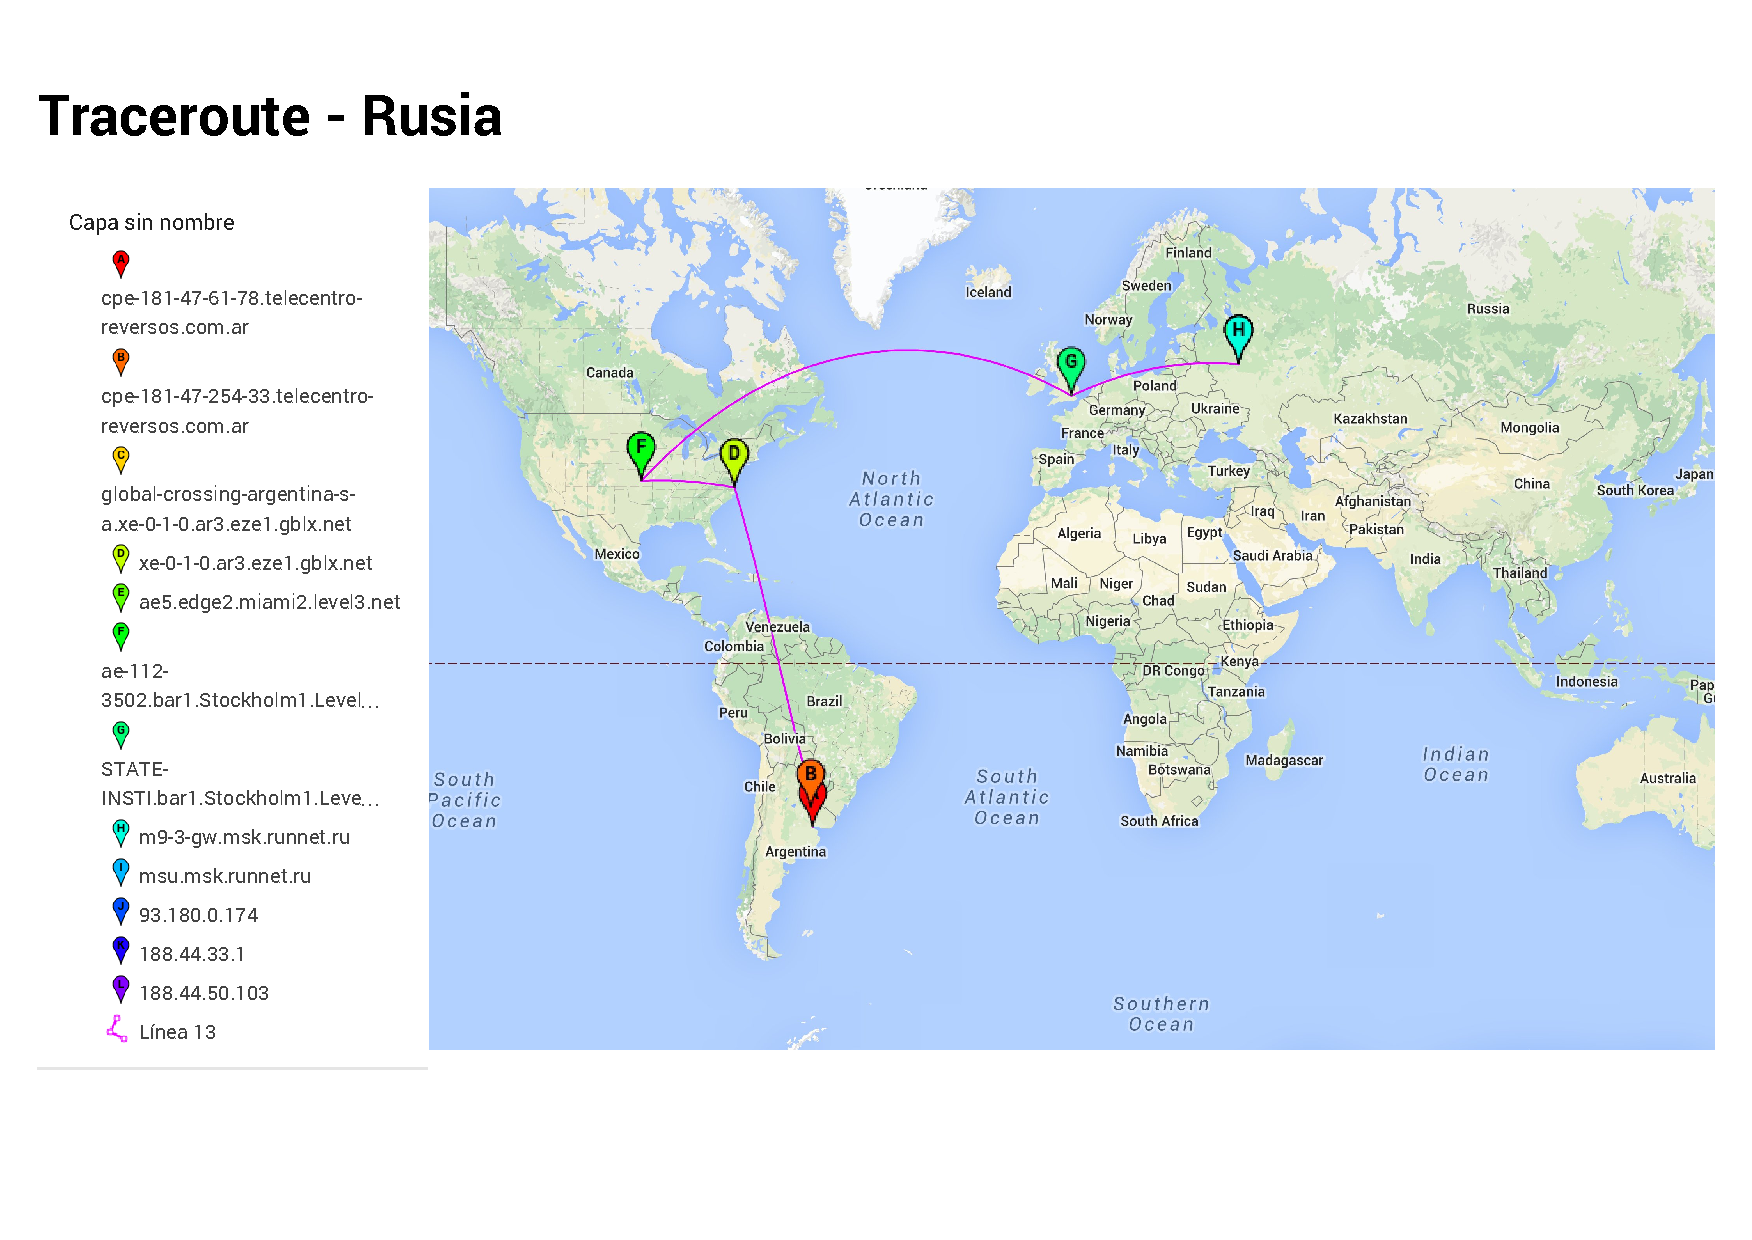
\includegraphics[width=0.8\textwidth]{mapas/rusia.png}}

\begin{center}
 \begin{tabular}{|l|l|l|l|l|}
    \hline
    Hop &Dirección IP &País &Ciudad &Lat - Long \\ \hline \hline
    1 & 192.168.1.1 &  &  & 0 0 \\ \hline
    2 & 10.20.128.1 &  &  & 0 0 \\ \hline
    3 & 181.47.254.33 & Argentina &  & -34.6033 -58.3817 \\ \hline
    4 & 208.178.195.210 & United States & Virginia & 36.8267 -76.0179 \\ \hline
    5 & 208.178.195.209 & United States & Virginia & 36.8267 -76.0179 \\ \hline
    6 & 4.68.111.121 & United States &  & 38 -97 \\ \hline
    7 & 4.69.158.245 & United States &  & 38 -97 \\ \hline
    8 & 4.69.158.245 & United States &  & 38 -97 \\ \hline
    9 & 213.242.110.198 & United Kingdom &  & 51.5 -0.13 \\ \hline
    11 & 194.85.40.229 & Russia &  & 55.75 37.6166 \\ \hline
    12 & 194.190.254.118 & Russia &  & 55.75 37.6166 \\ \hline
    13 & 93.180.0.174 & Russia & Moscow & 55.7522 37.6156 \\ \hline
    14 & 188.44.33.1 & Russia & Moscow & 55.7522 37.6156 \\ \hline
    15 & 188.44.50.103 & Russia & Moscow & 55.7522 37.6156 \\ \hline
 \end{tabular}
\end{center}

De acuerdo al mapa, se puede observar que el salto trasatlántico se da entre el host de Estados Unidos y el de Inglaterra. De acuerdo a 
la tabla se puede notar que el mismo sería entre el número $10$ y el $11$. Este salto presentará un valor alto de RTT a aquellos hops que se encuentren luego del número $11$ ya que se incorpora el tiempo de ida y vuelta por el enlace trasatlántico. Si nos dirijimos al gráfico de la página $10$, podremos observar con el hop que presenta un valor de ZRTT más alto es el $11$, por lo que se demuestra lo que ocurre en la realidad.    

\subsection{Universidad de Tokio}
\centerline{\includegraphics[width=0.8\textwidth]{mapas/Japon.png}}

\begin{center}
 \begin{tabular}{|l|l|l|l|l|}
    \hline
    Hop &Dirección IP &País &Ciudad &Lat - Long \\ \hline \hline
    1 & 192.168.0.1 &  &  & 0 0 \\ \hline
    2 & 190.195.209.1 & Argentina & Buenos Aires F.D. & -34.6033 -58.3816 \\ \hline
    6 & 200.89.165.77 & Argentina &  & -34.6033 -58.3817 \\ \hline
    7 & 200.89.165.1 & Argentina &  & -34.6033 -58.3817 \\ \hline
    8 & 200.89.165.250 & Argentina &  & -34.6033 -58.3817 \\ \hline
    9 & 206.165.31.213 & United States &  & 38 -97 \\ \hline
    10 & 67.16.139.18 & United States &  & 38 -97 \\ \hline
    11 & 64.212.107.98 & United States &  & 38 -97 \\ \hline
    12 & 129.250.3.172 & United States & Colorado & 39.6237 -104.8738 \\ \hline
    13 & 129.250.2.219 & United States & Colorado & 39.6237 -104.8738 \\ \hline
    14 & 129.250.7.69 & United States & Colorado & 39.6237 -104.8738 \\ \hline
    15 & 129.250.4.39 & United States & Colorado & 39.6237 -104.8738 \\ \hline
    16 & 129.250.6.90 & United States & Colorado & 39.6237 -104.8738 \\ \hline
    17 & 61.200.80.218 & Japan &  & 35.69 139.69 \\ \hline
    18 & 158.205.192.173 & Japan &  & 35.69 139.69 \\ \hline
    19 & 158.205.192.86 & Japan &  & 35.69 139.69 \\ \hline
    20 & 158.205.121.250 & Japan &  & 35.69 139.69 \\ \hline
    21 & 154.34.240.254 & Japan &  & 35.69 139.69 \\ \hline
    22 & 210.152.135.178 & Japan &  & 35.69 139.69 \\ \hline
 \end{tabular}
\end{center}

En el caso del salto del hop $8$ al $9$ puede presentarse como uno trasatlántico, ya que su tiempo de recorrida es bastante 
alto debido a la enorme distancia. Por otro lado, el que verdaderamente deberá responderse como un enlace trasatlántico es el que va del hop de Estados Unidos, el número $16$, al de Japón, el número $17$. Se observa en los gráficos comparativos de los valores del ZRTT correspondiente a cada hop, que el del número 15 corresponde al trasatlántico. En este caso, está ocurriendo lo mismo que se vio para la universidad de Alemania. Existe más de un camino posible para poder alcanzar el hop destino, y todos deberán pasar por el enlace trasatlántico. Puede darse tanto entre dos hops determinados o los consecutivos. 

\subsection{Universidad de Boston}
\centerline{\includegraphics[width=0.8\textwidth]{mapas/EEUU.jpg}}

\begin{center}
 \begin{tabular}{|l|l|l|l|l|}
    \hline
    Hop &Dirección IP &País &Ciudad &Lat - Long \\ \hline \hline
    3 & 181.47.254.85 & Argentina  &  & -34.6033 -58.3817 \\ \hline
    4 & 208.178.195.214 & United States & Virginia  & 36.8267 -76.0179 \\ \hline
    5 & 208.178.195.213 & United States & Virginia  & 36.8267 -76.0179 \\ \hline
    6 & 67.17.75.66 & United States  &  & 38 -97 \\ \hline
    7 & 4.68.111.121 & United States  &  & 38 -97 \\ \hline
    8 & 4.69.140.90 & United States & Florida  & 25.9372 -80.317 \\ \hline
    9 & 4.53.56.6 & United States & Massachusetts  & 42.2612 -71.4634 \\ \hline
    10 & 128.197.254.113 & United States & Massachusetts  & 42.3451 -71.0993 \\ \hline
    11 & 128.197.254.166 & United States & Massachusetts  & 42.3451 -71.0993 \\ \hline
    12 & 128.197.26.34 & United States & Massachusetts  & 42.3451 -71.0993 \\ \hline
 \end{tabular}
\end{center}

La universidad seleccionada se encuentra en Estados Unidos, por lo cual no existirá enlace trasatlántico, pero si se observa un salto importante de un host en Argentina a uno en Estados Unidos. Por lo tanto, en la sección anterior, se deberá observar al salto entre el TTL $3$ y el $4$ como el significativamente mayor con respecto a los restantes. 
Un problema importante presentado en el caso de esta universidad, es la cantidad de host intermedios que presentan un time-out. Se ve, por ejemplo, en los resultados del análisis de los valores standar para cada salto, que el salto entre el hop $5$ y el $6$ es significativamente mayor al restante. Sin embargo, al observar las distancias entre esos dos hops, la misma no es importante. Esto ocurre, como consecuencia a que el hop número $5$ no responde a muchos de los pedidos, por lo cual se genera un RTT promedio muy bajo. 
